\documentclass{amsbook}
\usepackage{graphicx} % Required for inserting images
\usepackage{float}
\usepackage[colorlinks=true,linkcolor=blue]{hyperref}
\usepackage{amssymb}
\usepackage{enumerate}
\usepackage{mathtools}
\usepackage{tikz}
\usepackage[answerdelayed]{exercise}
\usepackage{floatflt}
\usepackage{multicol}
\usepackage{subcaption}
\usepackage{tikz}
\usetikzlibrary{trees}
\usepackage[backend=biber,style=alphabetic,sorting=ynt]{biblatex}
\addbibresource{prob.bib}

\setlength{\parindent}{0pt}
\setlength{\listparindent}{0pt}
\renewcommand{\ExerciseHeaderTitle}{\quad\ExerciseTitle}
\renewcommand{\AnswerHeader}{\medskip\centerline{\emph{\ExerciseName\ \ExerciseHeaderNB} \smallskip}}
\renewcommand{\ExerciseHeader}{\medskip\ExerciseHeaderDifficulty{\emph{\ExerciseName\ \ExerciseHeaderNB\ExerciseHeaderTitle} \newline}}
\renewcommand{\QuestionNB}{(\alph{Question})\ }

\begin{document}

\title{Counting \& Probability:\\
    \Large Form V}

%\author{M. Martynovsky}
%\author{S. Chu}

\maketitle
\tableofcontents
\chapter*{Preface}
The following short booklet contains a collection of problems with solutions that roughly follow the topics typically covered in the Combinatorics and Probability unit of Form V mathematics classes at Ethical Culture Fieldston School. The hope is to provide a bank of problems of varying difficulty that will provide non-routine exercises as well as to record general themes and approaches to tackling these types of problems in general. Ideally these problems can be useful to all courses that cover these topics. Problems are roughly categorized by difficulty level and notated via *, **, or *** in increasing difficulty. We have adopted problems from memory, and from years of working with the material. The following references were consulted for problems as well as other considerations such as narrative structure in introducing various topics and thematic development of the material. \cite{mcirc}, \cite{aops}, \cite{hpn}, [more later].
\chapter{Logic \& Sets}

\section{Set Notation}

\begin{Exercise}[title={A few well known sets}, difficulty=0, label=s1]
Let $\mathbb{N}=\{1,2,3,4,\ldots\}$. These are the natural numbers or counting numbers. $\mathbb{Z}=\{\ldots, -2, -1, 0, 1, 2,3,\ldots\}$ is the set of integers. $\mathbb{Q}=\{p/q \, \big| \, p, q \in \mathbb{Z}\}$ is the set of rational numbers. $\mathbb{R}$ refers to the set of real numbers. $\mathbb{C}$ refers to the set of complex numbers.
    \Question Fill in the blank with $\subset$ or $\supset$. \quad $\mathbb{Z} \, \makebox[1em]{\hrulefill}\, \mathbb{N}$
    \Question Fill in the blank with $\subset$ or $\supset$. \quad $\mathbb{R} \, \makebox[1em]{\hrulefill} \, \mathbb{Q}$
    \Question Fill in the blank with $\subset$ or $\supset$. \quad $\mathbb{N} \, \makebox[1em]{\hrulefill} \, \mathbb{Q}$
    
    \hfill \emph{solution} \refAnswer{s1}
\end{Exercise}

\begin{Answer}[ref={s1}]
    The expression $A \subset B$ is read, the set $A$ is contained in the set $B$. Whereas the expression $A \supset B$ is read the set $A$ contains the set $B$.
    \begin{enumerate}
        \item $\mathbb{Z}\supset \mathbb{N}$
        \item $\mathbb{R}\supset \mathbb{Q}$
        \item $\mathbb{N} \subset \mathbb{Q}$
    \end{enumerate}
\end{Answer}

\begin{Exercise}[title={The cardinality of a set}, difficulty=0, label=s2]
Let $A=\{0,2,4,6,8, 10\}$, $B=\{4,8\}$, $C=\{1,3,5,7\}$, $D=\varnothing$ and $U=\{0,1,2,3,\ldots ,10\}$.
    \Question Calculate $|A|$.
    \Question Calculate $|D|$.
    \Question Calculate $|U|$.
    \Question Calculate $|B|$.
    \Question Give an argument as to why $B \subset A$ implies that $|B| \leq |A|$.
    
    \hfill \emph{solution} \refAnswer{s2} 
\end{Exercise}

\begin{Answer}[ref={s2}]
    \begin{enumerate}
        \item 6
        \item 0
        \item 11
        \item 2
        \item $B \subset A$ says that $B$ is a subset of $A$, which implies that every element of $B$ is an element of $A$, thus the number of elements in $B$ must be less than or equal to the number of elements in $A$.
    \end{enumerate}
\end{Answer}

\begin{Exercise}[title={Looking for an Element}, difficulty=0, label=s3]
    To indicate membership in a set $A$ we use the notation $x \in A$, which is read as $x$ is an element of the set $A$. For example let $E$ be the set of even integers. Then we can write that $4 \in E$, and $3 \notin E$. For each of the following sets: $\mathbb{Z}, \mathbb{Q}, \mathbb{R}$, and $\mathbb{C}$, choose a different element that you know is in the set, and use it to write an expression that states it is a member of the given set. 

    \hfill \emph{solution} \refAnswer{\ExerciseLabel}
\end{Exercise}

\begin{Answer}[ref={s3}]
    
\end{Answer}

\begin{Exercise}[title={Using set notation}, difficulty=1, label=s4]
    You can describe a set by giving a condition that elements must satisfy to be a member of the set. For examples the even numbers can be describe as the set of integers that are divisible by 2. $\{x\in \mathbb{Z} \, \big| \, x=2n \, , n\in\mathbb{Z}\}$, or $\{x \in \mathbb{Z} \, \big| \, 2|x\}$. 
    \Question Describe the set of odd numbers using set notation.
    \Question Describe the set of multiples of 5 using set notation.
    \Question Describe the set of the real numbers in the interval $[3,10]$ using set notation. 
    
    \hfill \emph{solution} \refAnswer{s4}   
\end{Exercise}

\begin{Answer}[ref={s4}]
    \begin{enumerate}
        \item $\{x \in \mathbb{Z} \:\big| \: x=2n-1 \, n\in\mathbb{Z}\}$\\
        \item $\{x \in \mathbb{Z} \: \big| \: x=5n \, n\in\mathbb{Z}\}$\\
        \item $\{x \in \mathbb{R} \: \big| \: 3\leq x\leq 10\}$\\
    \end{enumerate}
\end{Answer}

\begin{Exercise}[title={Distance of 2}, difficulty=1, label=s5]
    Let $A=\{(x,y) \, \big| \, x,y \in \mathbb{Z} \mbox{ and } x^2+y^2=2\}$. Enumerate the elements of $A$. 
    
    \hfill \emph{solution} \refAnswer{s5}
\end{Exercise}

\begin{Answer}[ref={s5}]
    $A$ is the set of lattice points that lie on the circle of radius 2 centered at the origin. $A =\{(-2,0);(0,2); (0,-2); (2,0)\}$.
\end{Answer}

\begin{Exercise}[title={Still distance of 2?}, difficulty=2, label=s6]
    Enumerate the elements of each set described below.
        \begin{enumerate}
            \item $A=\{(x,y) \big| \, x,y \in \mathbb{Z} \mbox{ and } |x|+|y|=2\}$\\
            \item $B=\{(x,y) \big| \, x,y \in \mathbb{Z} \mbox{ and } \max(x,y)=2\}$
        \end{enumerate}
        \hfill \emph{solution} \refAnswer{s6}
\end{Exercise}

\begin{Answer}[ref={s6}]
    
\end{Answer}


\section{Operations with Sets and Venn Diagrams}

\begin{Exercise}[title={Visualizing Some Sets}, difficulty=0, label=vd1]
    Let $U$ be the universal set. Draw a clearly labeled Venn Diagrams (one for each condition) of sets $A$ and $B$ such that:    
    \Question $A \cap B = B$
    \Question $A \cup B =U$
    \Question $A \cup B= A$
    \Question $A \cap B =\varnothing$

    \hfill \emph{solution} \refAnswer{\ExerciseLabel}
\end{Exercise}

\begin{Answer}[ref={vd1}]
    
\end{Answer}

\begin{Exercise}[title={Visualizing Some Sets II}, difficulty=0, label=vd2]
    Let $U$ be the universal set. Draw a clearly labeled Venn Diagram of the sets $A$, $B$ and $C$ such that:
    \Question $A \cap B \cap C$, $A \cap B \cap C^c$ in nonempty, but $C \subset (A \cup B)$.
    \Question more soon

    \hfill \emph{solution} \refAnswer{\ExerciseLabel}    
\end{Exercise}

\begin{Answer}[ref={vd2}]
    
\end{Answer}

\begin{Exercise}[title={Intersections II}, difficulty=1, label=os1]
    \Question Explain why if $A \subset B$ then $A \cap B=A$.
    \Question Explain why $A \cap A^c = \varnothing$.
    \Question Explain why $|A \cap B| \leq \min\{|A|, |B|\}$.
\hfill \emph{solution} \refAnswer{\ExerciseLabel}
\end{Exercise}

\begin{Answer}[ref={os1}]
    
\end{Answer}


\begin{Exercise}[title={Multiples of a Number}, difficulty=2, label=os2]
    Let $n\mathbb{Z}$ denote the multiples of $n.$ For example $5\mathbb{Z}=\{\ldots,-5,0,5,10,15,20,\ldots\}$.
    \Question How would you best describe the set $3\mathbb{Z} \cap 6\mathbb{Z}$?
    \Question How would you best describe the set $3\mathbb{Z} \cap 10\mathbb{Z}$?
    \Question How would you best describe the set $a\mathbb{Z} \cap b\mathbb{Z}$?

    \hfill \emph{solution} \refAnswer{\ExerciseLabel}
\end{Exercise}

\begin{Answer}[ref={os2}]
    
\end{Answer}

\begin{Exercise}[title={Multiples of a Number II}, difficulty=2, label=os3]
    How would you best describe the set $a\mathbb{Z} \cup b\mathbb{Z}$?

    \hfill \emph{solution} \refAnswer{\ExerciseLabel}
\end{Exercise}

\begin{Answer}[ref={os3}]
    
\end{Answer}

%%%

\section{Pigeon Hole Principle}

\begin{Exercise}[title={Initial Twins}, difficulty =1, label=php2]
    Show that among the faculty and students at Fieldston Upper and Middle, there are at least two people with the same first and last initials.

    \hfill \emph{solution} \refAnswer{\ExerciseLabel}
\end{Exercise}

\begin{Answer}[ref={php2}]
    
\end{Answer}

\begin{Exercise}[title={Not a Flush}, difficulty =1, label=php3]
    Show that if you pick 5 random cards from a typical deck of 52 cards that at least two of them will be the same suit.

    \hfill \emph{solution} \refAnswer{\ExerciseLabel}
\end{Exercise}

\begin{Answer}[ref={php3}]
    
\end{Answer}

\begin{Exercise}[title={Partitions of a Number}, difficulty=1, label=php4]
    Show that if you pick any five numbers from the set of integers $1\leq x \leq 8$ that two of the numbers must sum to 9.

    \hfill \emph{solution} \refAnswer{\ExerciseLabel}
\end{Exercise}

\begin{Answer}[ref={php4}]
    
\end{Answer}

\begin{Exercise}[title={A Friendly Party}, difficulty=2, label=php5]
    Show that at a party that has at least 2 people attending it, that there must be two people what have the same number of friends. Assume being a friend is a symmetric relationship. 

    \hfill \emph{solution} \refAnswer{\ExerciseLabel}
\end{Exercise}

\begin{Answer}[ref={php5}]
    
\end{Answer}

\begin{Exercise}[title={Orange Great Circles}, difficulty=2, label =php6]
    Show that if you draw five points on an orange that you can always cut the orange in half through the center so that four points lie on one hemisphere. Here assume that points along the cut are on both hemispheres.

    \hfill \emph{solution} \refAnswer{\ExerciseLabel}
\end{Exercise}

\begin{Answer}[ref={php6}]
    
\end{Answer}

\begin{Exercise}[title={Finding Points}, difficulty=3, label=php1]
    Show that given any five points inside an equilateral triangle of side length two, that at least two points are at most one away from one another. 
    \hfill \emph{solution} \refAnswer{php1}
\end{Exercise}

\begin{Answer}[ref={php1}]
    If you draw the midsegments of the triangle you will create 4 congruent triangles of side length one. Given any five points at least two of the them will be on or inside one of the triangle.
\end{Answer}

\begin{Exercise}[title={Another Chessboard Problem}, difficulty=2, label=php7]
    Show that you cannot cover a chessboard with dominoes that each cover exactly 2 squares on the chessboard if the chessboard is missing two squares on opposite diagonal corners.
    \begin{figure}[H]
        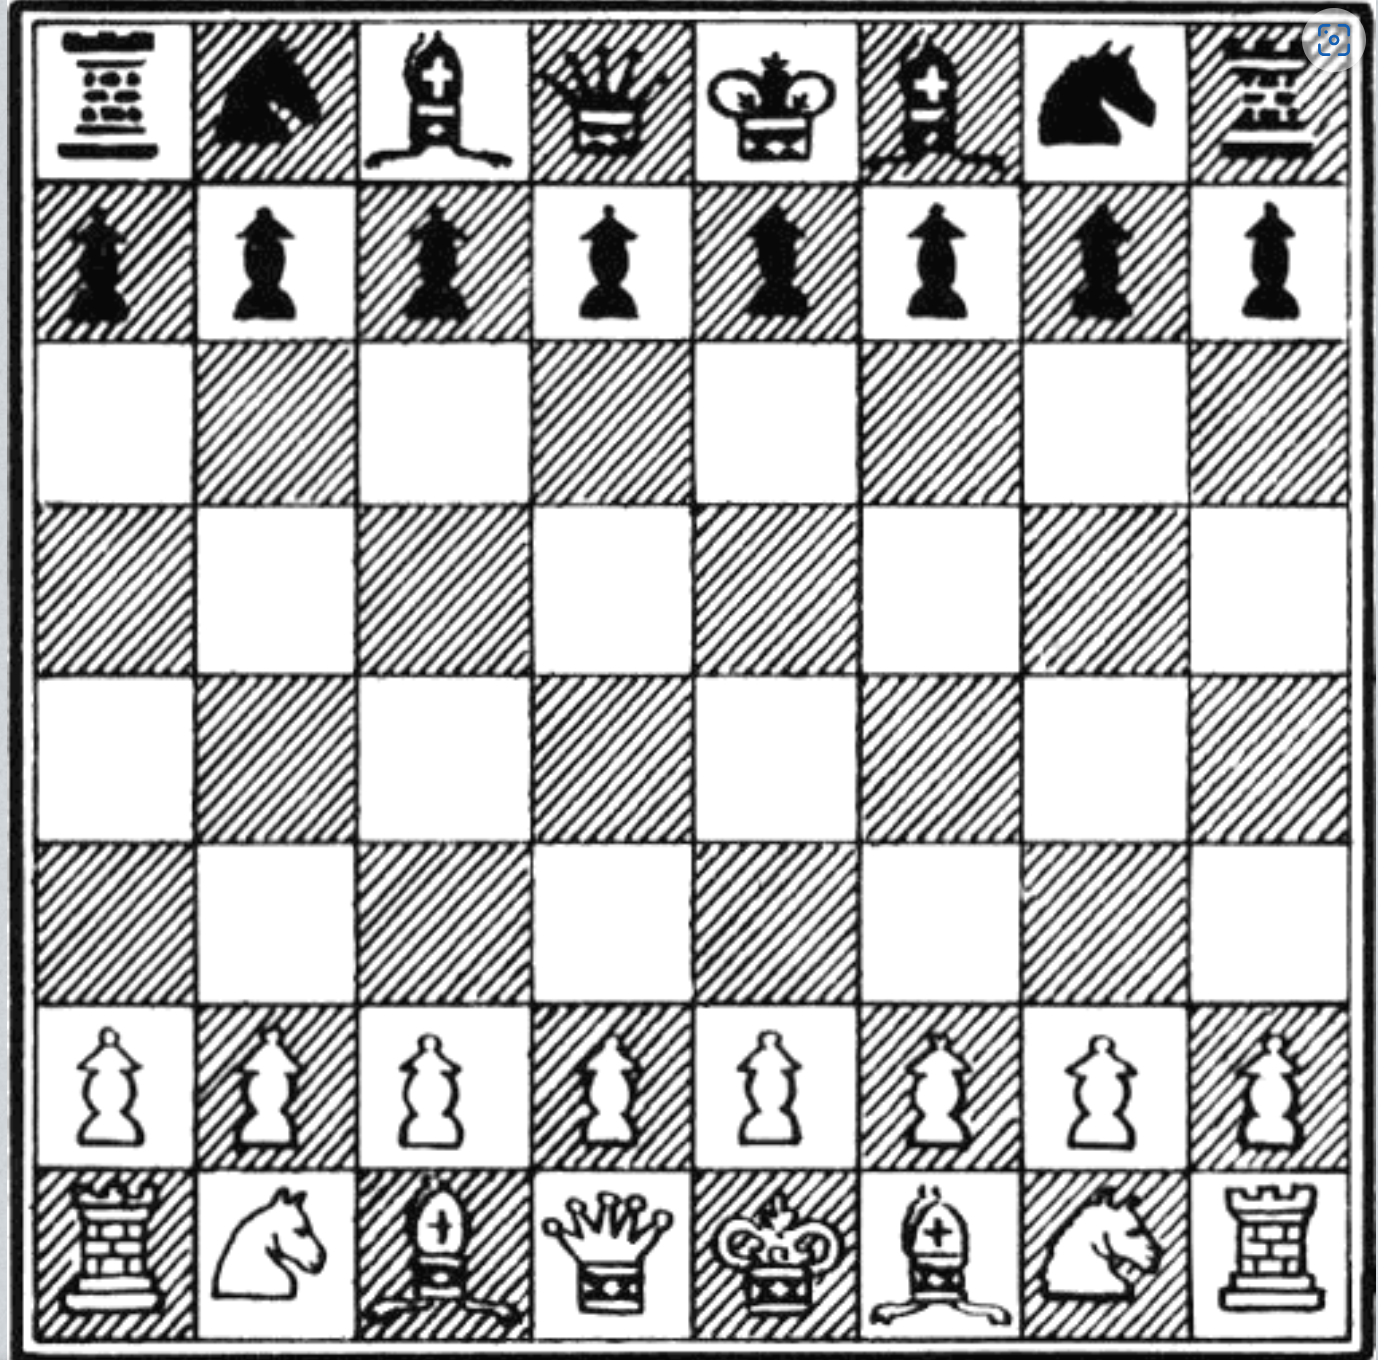
\includegraphics[width=.3\linewidth]{m.png}
    \end{figure}
\end{Exercise}

\begin{Answer}[ref={php7}]
    
\end{Answer}

\chapter{Combinatorics}
%The section on counting and probability usually follows the unit on sequences and series. 

\section{Multiplication Principle}

\begin{Exercise}[title={Making Choices...},difficulty=0, label=m1]
    If you have 4 sweaters and 2 pairs of jeans, how many different outfits can you make? \hfill \emph{solution} \refAnswer{\ExerciseLabel} 
    \begin{figure}[H]
        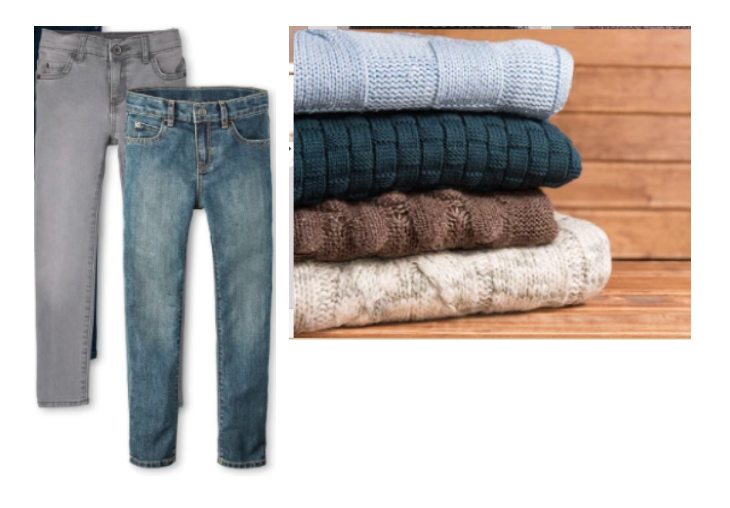
\includegraphics[width=.5\linewidth]{h.png}
    \end{figure}
    
\end{Exercise}

\begin{Answer}[ref={m1}]
    There are 8 possible outfits. You have four choices of sweater, and for each of these you have a subsequent 2 choices for jeans. You can also view this using a tree diagram that illustrates the available choices. 
    % Set the overall layout of the tree
\tikzstyle{level 1}=[level distance=3cm, sibling distance=2cm]
\tikzstyle{level 2}=[level distance=4.5cm, sibling distance=1cm]

% Define styles for nodes
\tikzstyle{shirt} = [fill=green, rectangle, rounded corners]
\tikzstyle{jean} = [fill=blue!20, rectangle, rounded corners]
\tikzstyle{start}=[circle, minimum width=2pt, fill, inner sep=0pt]
% Make the tree
\begin{tikzpicture}[grow=right]
\node[start] {}
    child {
        node[shirt] {sweater 1}% This is the first of four sweaters
            child {
                node[jean] {jeans 1}
            }
            child {
                node[jean] {jeans 2}
            }
    }
    child {
        node[shirt] {sweater 2}
            child {
                node[jean] {jeans 1}
            }
            child {
                node[jean] {jeans 2}
            }
    }
    child {
        node[shirt] {sweater 3}
            child {
                node[jean] {jeans 1}
            }
            child {
                node[jean] {jeans 2}
            }
    }
    child {
        node[shirt]{sweater 4}
            child{
                node[jean]{jeans 1}
            }
            child{
                node[jean]{jeans 2}
            }
    };
\end{tikzpicture}
\end{Answer}

\begin{Exercise}[title={Choices with a Restriction}, difficulty=1, label=m2]
    You have 4 sweaters. One blue, one green, one brown and one white sweater. You have 2 pairs of jeans. One pair is blue and the other is gray. How many different outfits can you make if you don't want the sweater and jeans to be the same color? 
    
    \hfill \emph{solution} \refAnswer{\ExerciseLabel}
\end{Exercise}

\begin{Answer}[ref={m2}]
    There are 7 outfits. We already know there are 8 total possible outfits, and there is only one that has matching colors.
\end{Answer}

\begin{Exercise}[title={Rearrangements}, difficulty=0, label=m3]
    In how many ways can 7 people line up in a cafeteria line? \hfill \emph{solution} \refAnswer{\ExerciseLabel}
    
    \begin{figure}[H]
        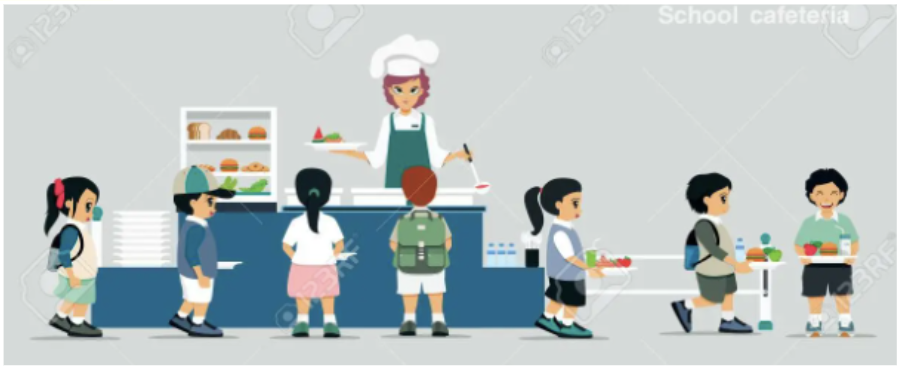
\includegraphics[width=.5\linewidth]{j.png}
    \end{figure}
\end{Exercise}

\begin{Answer}[ref={m3}]
    5040. We can treat each spot in line as a choice. For the first person in line there are 7 possibilities, for the second there are only 6 as you have already place 1 or the 7 people first in line. For the third there are 5 possible choices and so on. So using the multiplication principle over 7 choices we have $7\cdot 6\cdot 5\cdot 4\cdot 3\cdot 2\cdot 1=5040$ possible lineups.
\end{Answer}

\begin{Exercise}[title={Rearrangements with a restriction}, difficulty=1, label=m4]
    In how many ways can 7 people line up in a cafeteria line if Jamie and Jean always go to lunch together?

    \hfill \emph{solution} \refAnswer{\ExerciseLabel}
\end{Exercise}

\begin{Answer}[ref={m4}]
    1440. In this situation we can think of Jamie and Jean as one unit, so we are only rearranging 6 places. After we count the rearrangements of 6 places we then need to make the choice of who is in front of who in our unit of two, Jamie or Jean. So we get $6! \cdot 2=1440$.
\end{Answer}

\begin{Exercise}[title={License Plates}, difficulty =1, label =m5]
   \Question How many different license plates can be made using 3 letters followed by 4 numbers, if repetition is allowed?
    \begin{figure}[H]
        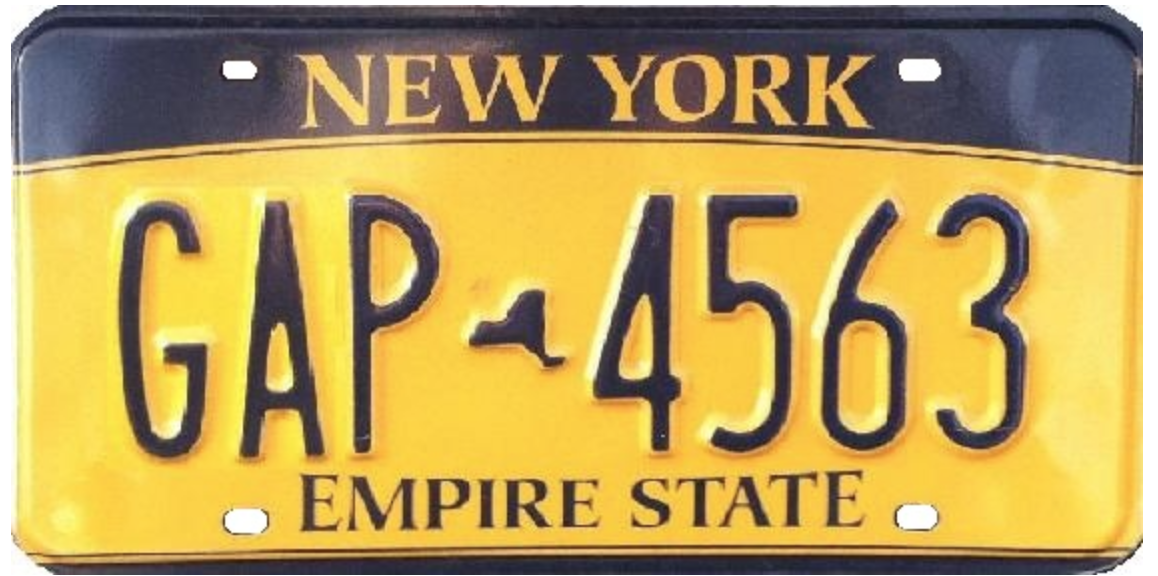
\includegraphics[width=.4\linewidth]{k.png}
    \end{figure}
    \Question How many different license plates can be made using 3 letters followed by 4 numbers, if repetition is not allowed?
    \Question How many different license plates can be made using 3 letters followed by 4 numbers, if repetition is allowed but the number 0 and the letter O are not?
    
    \hfill \emph{solution} \refAnswer{\ExerciseLabel}
\end{Exercise}

\begin{Answer}[ref={m5}]
    TBW
\end{Answer}

\begin{Exercise}[title={An Excuse to Play Chess}, difficulty=0, label=m8]
    In how many ways can you place a white rook and a black rook on a chessboard so that they are not threatening one another?

    \hfill \emph{solution} \refAnswer{\ExerciseLabel}
\end{Exercise}

\begin{Answer}[ref={m8}]
    We can place the first rook anywhere so there are 64 options. This rook is now sitting on one square and threatening 14 other squares so there are $64-15=49$ squares available for the other rook such that it is not being attached by the first rook. Hence there are $64 \cdot 49=3,136$ ways to place the two rooks.
\end{Answer}

\begin{Exercise}[title={Palindromes}, difficulty=1, label=m6]
    \Question How many 2 digit palindromes are there?
    \Question How many 3 digit palindromes are there?

\hfill \emph{solution} \refAnswer{\ExerciseLabel}
\end{Exercise}

\begin{Answer}[ref={m6}]
    \begin{enumerate}
        \item Two digit palindromes have the form `aa' such that $a=\{1,2,3,\ldots, 9\}$. So there are 9 possibilities.
        \item Three digit palindromes have the form `aba' where $b$ can be any single digit, but again $a$ is restricted as before. Using the multiplication principle there are 10 options for $b$ and 9 options for $a$. So there are 90 options.
    \end{enumerate}
\end{Answer}

\begin{Exercise}[title={Palindromes II}, difficulty=2, label=m7]
    \Question How many 4 digit palindromes are multiples of 5?
    \Question How many 4 digit palindromes are multiples of 3?
    \Question How many 4 digit palindromes are multiples of 15?

    \hfill \emph{solution} \refAnswer{\ExerciseLabel}
\end{Exercise}

\begin{Answer}[ref={m7}]
    
\end{Answer}

\section{Addition Principle}

\begin{Exercise}[title={Roads to Rome}, difficulty=0, label=ap1]
    In Math land there are four towns $A$, $B$, $C$, and $D$. There are one way roads built between all of the cities as depicted in the figure below. How many ways are there to drive from town A to town C?
    \begin{figure}[H]
        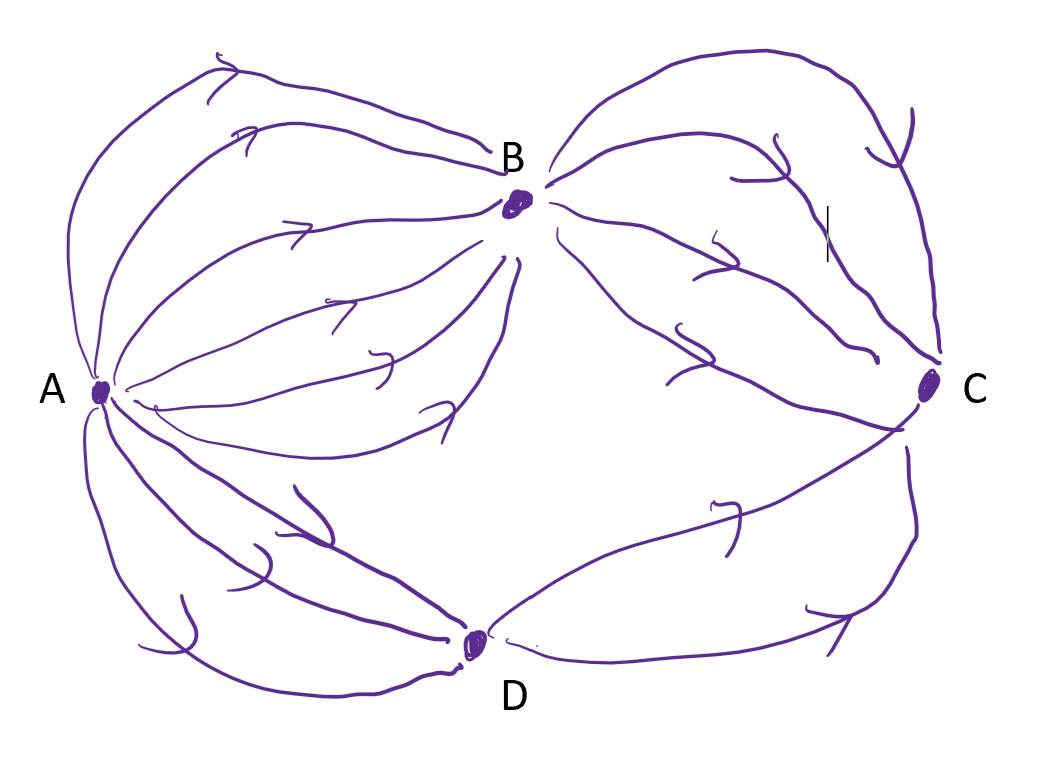
\includegraphics[width=.4\textwidth]{o.png}
    \end{figure}
    \hfill \emph{solution} \refAnswer{\ExerciseLabel}
\end{Exercise}

\begin{Answer}[ref={ap1}]
    Here we combine the multiplication principle with the addition principle. You can travel from $A$ to $C$ either by passing through $B$ or $D$. For the route $A\to B \to C$ there are $6\cdot 4=24$ paths. For the route $A \to D \to C$ there are $3\cdot 2 =6$ paths. This gives a total of 30 paths from town $A$ to town $C$.
\end{Answer}

\begin{Exercise}[title={Digits of the same Parity}, difficulty =1, label=ap2]
    How many 6 digit numbers have either all even digits or all odd digits?

    \hfill \emph{solution} \refAnswer{\ExerciseLabel}
\end{Exercise}

\begin{Answer}[ref={ap2}]
    There are two cases, the case of all even digits and all odd digits. We will use the multiplication principles to tally the possibilities for each case and then sum the results. For the even case we have $4\cdot 5^5$ possibilities and for the odd case we have $5^6$ possibilities. So in total there are $5^5(4+5)=9\cdot 5^5=28,125$ numbers.
\end{Answer}

\begin{Exercise}[title={An Excuse to Play Chess II}, difficulty=2, label=ap3]
    How many ways are there to place a black king and a white king on a chess board such that they are not attacking one another?

    \hfill \emph{solution} \refAnswer{\ExerciseLabel}
\end{Exercise}

\begin{Answer}[ref={ap3}]
    
\end{Answer}

\section{Complements}

\begin{Exercise}[title={Phone Numbers?}, difficulty=2, label=co1]
    How many 7 digit numbers have at least one digit that is a 5?
    
\end{Exercise}

\begin{Exercise}[title={Phone Numbers II?}, difficulty =2, label=co2]
    How many 7 digit numbers have at least one odd digit?
\end{Exercise}

\section{Permutations}

\begin{Exercise}[title={Rearrangements Again}, difficulty=0, label=p1]
    \Question You have three colored marbles. One yellow, one red and one green. In how many ways can you place them in a row?
    \Question If all three marbles are yellow, in how many ways can you place them in a row?
    \Question If two marbles are yellow and one is red, in how many ways can you place them in a row?
\end{Exercise}

\begin{Exercise}[title={Marbles}, difficulty=1, label=p2]
    You have five marbles. Four are blue and one is red. In how many ways can you place them in a row?
    \begin{figure}[H]
        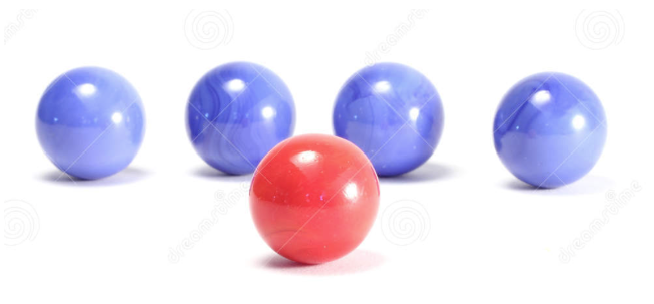
\includegraphics[width=.4\linewidth]{n.png}        
    \end{figure}
\end{Exercise}

\begin{Exercise}[title={Marbles II}, difficulty=2, label=p3]
    \Question You have five marbles. Three are blue and two are red. In how many ways can you place them in a row?
    \Question You have 10 marbles. Eight are blue and two are red. In how many ways can you them in a row?
    \Question You have 8 identical marbles. In how many different ways can you distribute them into 3 containers?
    \Question You have 20 identical shirts. In how many different ways can you distribute them into 4 drawers?

\hfill \emph{solution} \refAnswer{\ExerciseLabel}
\end{Exercise}

\begin{Answer}[ref={p3}]
    
\end{Answer}

\begin{Exercise}[title={An Ice Cream Cone a Day}, difficulty=1, label=p4]
    
\end{Exercise}

\section{Combinations}

\begin{Exercise}[title={Paths on a Grid},difficulty=1, label=c1]
The grid below represents the streets of a city. You are traveling from point $X$ to point $Y$ by moving either to the right or down. How may different routes are there from $X$ to $Y$? \hfill \emph{solution} \refAnswer{\ExerciseLabel} 
    \begin{figure}[H]
    \begin{subfigure}{0.45\textwidth}
        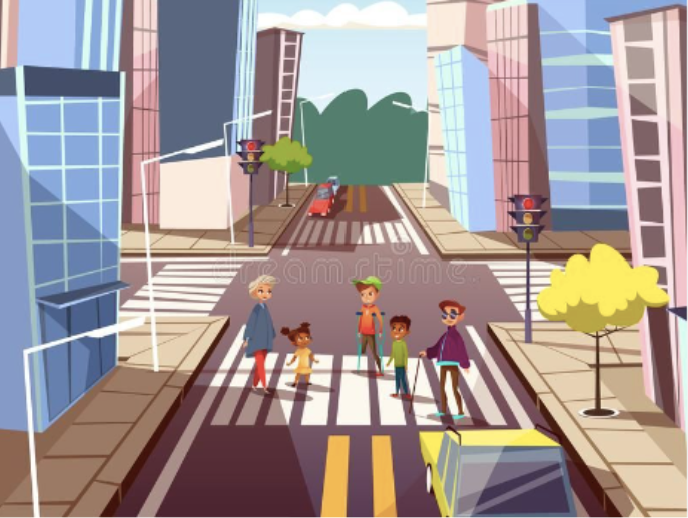
\includegraphics[width=0.9\linewidth, height=4cm]{a.png}  
    \end{subfigure}
    \begin{subfigure}{0.45\textwidth}
      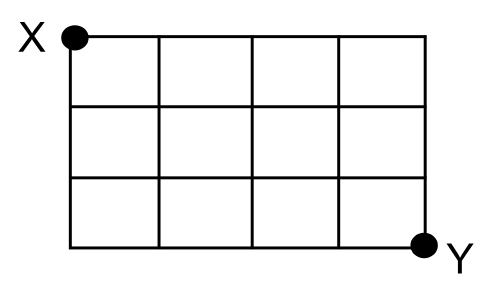
\includegraphics[width=0.9\linewidth, height=3cm]{b.png}
    \end{subfigure}
    \end{figure}
\end{Exercise}

\begin{Answer}[ref={c1}]
    There are 35 paths. You can arrive at this answer by recognizing that each path is composed of 7 parts. Four of which are to the right and 3 of which are down. You can count this either as ${7 \choose 4}$, choosing which 4 parts will be to the right, ${7 \choose 3}$, choosing which 3 parts will be down, or by calculating, $\dfrac{ 7!}{(4!)(3!)}$ where you count the rearrangements of all 7 parts dividing out by repetitions of right and down.
\end{Answer}

\begin{Exercise}[title={Paths on a Grid II}, difficulty=2, label=c2]
    Again the grid below represents the streets of a city. You are still traveling from $X$ to $Y$, but this time you must avoid passing through point $A$. How many routes are there from $X$ to $Y$ that do not pass through $A$? \hfill \emph{solution} \refAnswer{\ExerciseLabel}
    \begin{figure}[H]
     \centering
        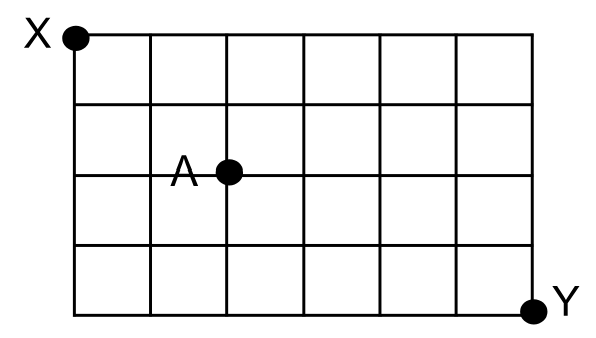
\includegraphics[scale=.55]{c.png}
    \end{figure}
\end{Exercise}

\begin{Answer}[ref={c2}]
    There are 120 paths. In this problem we want to avoid the point $A$. So we can first tally all the routes from $X$ to $Y$ as $10 \choose 6$, and then we take away all the paths that pass through $A$. There are two pieces to this journey. The trip from $X$ to $A$ can be done ${4 \choose 2} = 6$ ways, and the trip from $A$ to $Y$ can be done in ${6 \choose 2} =15$ ways. Using the multiplication counting principle this means there are $6\cdot 15 =90$ ways to go from $X$ to $Y$, passing through $A$. If we want to avoid point $A$ that means we will only have $210-90=120$ paths.
\end{Answer}

\begin{Exercise}[title={Paths on a Grid III}, difficulty=2, label=c3]
    In this situation, you cannot use the path from $A$ to $B$, but still may pass through point A and point B. How many routes are there connecting $X$ to $Y$? 
    
    \hfill \emph{solution} \refAnswer{\ExerciseLabel}
    \begin{figure}[H]
        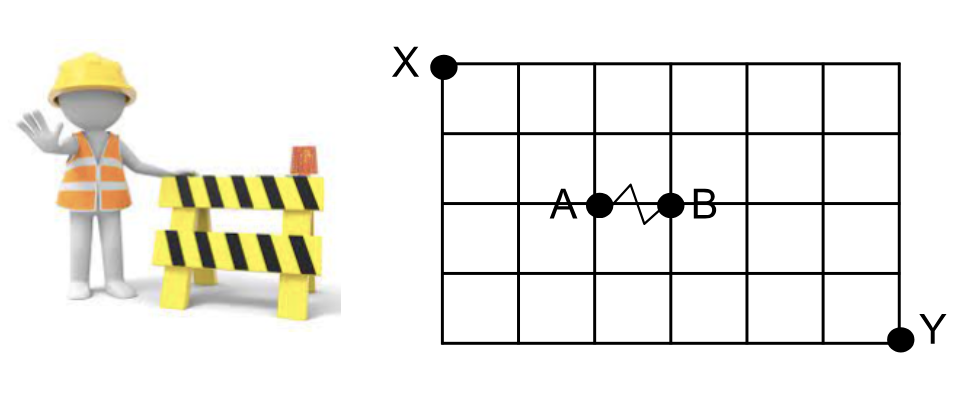
\includegraphics[width=.6\linewidth]{d.png}
    \end{figure}
\end{Exercise}

\begin{Answer}[ref={c3}]
    There are 150 paths. We start with 210 total paths from $X$ to $Y$. Then we remove all the paths that go from $X$ to $A$, then take $AB$, and then go from $B$ to $Y$. Enumerating those paths, we get ${4 \choose 2} =6$ paths from $X$ to $A$. There is only one way to get from $A$ to $B$, and then ${5\choose 2}=10$ ways to go from $B$ to $Y$. Using the multiplication principles there are a total of 60 paths that are not allowed by the road block. So there are a total of 210-60=150 paths from $X$ to $Y$ that avoid the road $AB$.
\end{Answer}

\begin{Exercise}[title ={Paths on a Grid IIIb}, difficulty=2, label=c4]
    You are in the same situation as the previous exercise, but this time you are not allowed to pass through $A$ or $B$ on your from $X$ to $Y$. How many routes meet these new conditions? How do Paths on a Grid problems II and III confirm what we intuitively understand about the difference in closing an intersection vs. closing a street (but no intersections).  \hfill \emph{solution} \refAnswer{\ExerciseLabel}
\end{Exercise}

\begin{Answer}[ref={c4}]
    There are 20 paths. Again we start with the 210 total paths from $X$ to $Y$. This time we must remove all paths from $X$ to $A$ followed by $A$ to $Y$ \emph{and} all paths that go from $x$ to $B$ followed by $B$ to $Y$.\\
    There are ${4\choose 2}{6\choose 2}=6\cdot 15=90$ paths that go $x$ to $A$ to $Y$. There are ${5\choose 2}{5\choose 2}=10\cdot 10=100$ paths that go $x$ to $B$ to $Y$. So if we have to avoid $A$, $B$ and the path $AB$ there are only $210-90-100=20$ paths.
\end{Answer}

\begin{Exercise}[title={Paths from Cell-to-Cell}, difficulty=1, label=c5]
    How many paths are there from the center of the bottom-most cell farthest to the left that end at the top-most cell farthest to the right, if you are restricted to moving either up or to the right? \hfill \emph{solution} \refAnswer{\ExerciseLabel}
    \begin{figure}[H]
        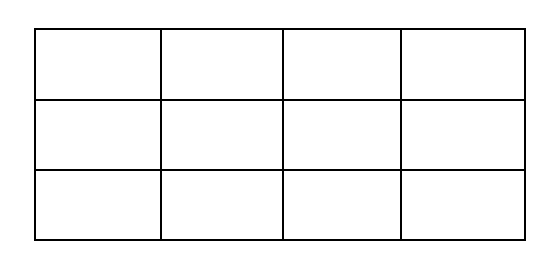
\includegraphics[width=.4\linewidth]{e.png}
    \end{figure}  
\end{Exercise}

\begin{Answer}[ref={c5}]
    There are ${5 \choose 2} =10$ paths. This is the same the same reasoning as the paths on a grid problems except instead of looking at the intersections points of the grid lines, we are looking at the centers of each rectangle.
\end{Answer}

\begin{Exercise}[title={Cell-to-Cell II}, difficulty=1, label=c6]
    How many paths are there from the center of the bottom-most cell farthest to the left that end at the top-most cell farthest to the right, if you are restricted to moving either up or to the right, and must avoid the black colored cell?
    
    \hfill \emph{solution} \refAnswer{\ExerciseLabel}
    \begin{figure}[H]
        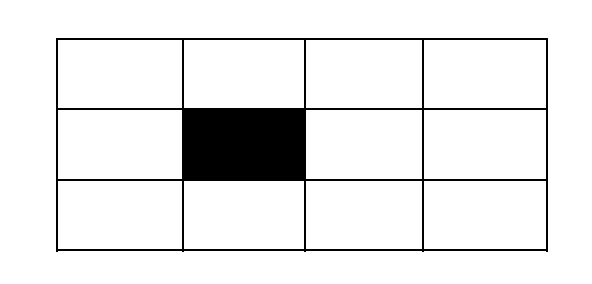
\includegraphics[width=.4\linewidth]{f.png}
    \end{figure}
\end{Exercise}

\begin{Answer}[ref={c6}]
    There are 4 paths. We can tackle this much as we did with the grid problems just by taking the total number of paths ${5 \choose 2}=10$ and subtracting the paths that contain the black cell, of which there are $(2)(3)=6$ paths. It would be good to also present an alternative way of solving by counting the number of paths from the lower left corner to each adjacent cell. We will use the fact that the number of paths to a given cell will be the sum of the number of paths for the cell below and the cell to the left. This is because all paths consist only of moves to the right or moves up. Doing this we can amend the figure as follows to see there are a total of 4 paths.
        \begin{figure}[H]
            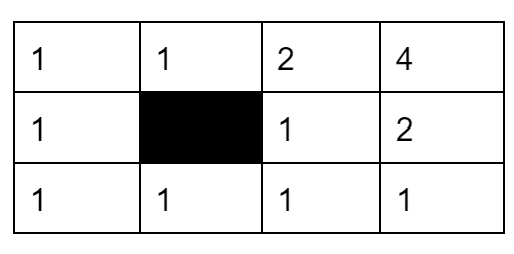
\includegraphics[width=.4\linewidth]{i.png}
        \end{figure}
\end{Answer}

\begin{Exercise}[title={Cell-to-Cell III}, difficulty=2, label=c7]
    \Question How many paths are there moving from the center of the cell in the bottom left corner to the the cell in the upper right corner, if you are restricted to moving either up or to the right and must avoid all the black colored cells?
     \begin{figure}[H]
        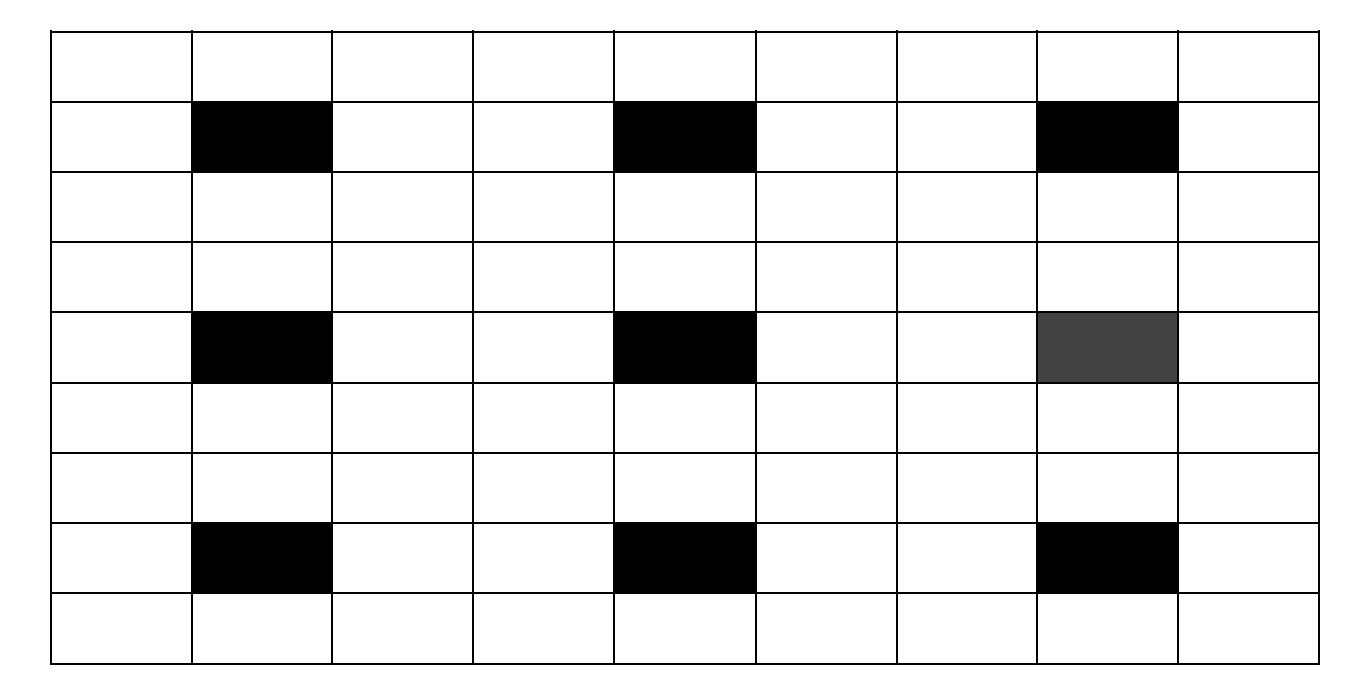
\includegraphics[width=.8\linewidth]{g.png}
    \end{figure}
    \Question Explain why it is sufficient to know the number of ways to get from the cell in the bottom left corner to each of the white cells along the diagonal that runs from the upper left corner to lower right corner, in order to determine the answer to the previous question. \hfill \emph{solution} \refAnswer{\ExerciseLabel}
\end{Exercise}

\begin{Answer}[ref={c7}]
    You can make your way around the diagram counting the paths from the bottom left corner to each white cell, much like the previous problem. This is a long winded process that you can abbreviate by only counting up to the white cells on the diagonals. For each white cell along the diagonal, due to symmetry, there are the same number of paths from the bottom left corner cell to the diagonal as there are from the upper right corner cell to the diagonal, thus you can count the total number of paths by squaring the number of paths to each diagonal cell, and summing them getting 678 paths.
\end{Answer}

\chapter{Probability}

\section{Basic Probability}

\section{Independent Events}

\begin{Exercise}[title={Newton talks with Pepys}, difficulty=2, label=ie1]
    Determine which of the following events is most likely by calculating the probability of each.
        \begin{enumerate}
            \item Six fair dice are rolled independently and at least one 6 appears.
            \item twelve fair dice are rolled independently and at least two 6's appear.
            \item eighteen fair dice are rolled independently and at least three 6's appear.
        \end{enumerate}

        \hfill \emph{solution} \refAnswer{\ExerciseLabel}
\end{Exercise}

\begin{Answer}[ref={ie1}]
    The first situation has probability $1-(5/6)^6=\dfrac{31031}{46656}\approx 0.6651$. Using a similar idea and we can find the probability of the second as $1-(5/6)^{12}-12(1/6)(5/6)^{11} \approx 0.6187$, and lastly the probability of the third event is $1-(5/6)^{18}-18(1/6)(5/6)^{17}-{18 \choose 2}(1/6)^2(5/6)^{16} \approx 0.5973$.
\end{Answer}

\begin{Exercise}[title={Pascal's Problem}, difficulty=2, label=ie2]
    When rolling two fair dice, how many rolls must be allowed to have a better than even chance of getting 2 sixes at least once?
\end{Exercise}

\begin{Answer}[ref={ie2}]
    
\end{Answer}


\section{Conditional Probability}

\section{Bayes' Theorem}

\section{Binomial Probability}

\section{Expected Value}

\begin{Exercise}[title={Dice}, difficulty=1, label=ev1]
    What is the expected value of one roll of a die.
    \begin{figure}[H]
        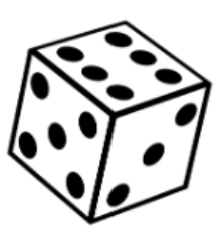
\includegraphics[width=.2\linewidth]{l.png}
    \end{figure}

    \hfill \emph{solution} \refAnswer{\ExerciseLabel}
\end{Exercise}

\begin{Answer}[ref={ev1}]
    The expected value is the sum of the products of the possible values of the random variable and their likelihood. So we get $\dfrac{1+2+3+4+5+6}{6}=21/6=7/2=3.5$ 
\end{Answer}

\begin{Exercise}[title={Newton and Pepys gamble}, difficulty =2, label = ev2]
    You are given the option to play a game where if you roll six fair dice and at least one of them shows a 6 you win 10 dollars. What is a fair price to play this game? Fair meaning the expected value of one play is zero.
\end{Exercise}

\begin{Answer}[ref={ev2}]
    
\end{Answer}

\begin{Exercise}[title={A Game with a Biased Coin}, difficulty=1, label=ev3]
    You are playing a game where you win 2 dollars if a biased coin lands heads and lose 1 dollar if it lands tails. The coin will land heads with probability 3/4. What is the expected value of one play of this game?
    
\end{Exercise}

\begin{Answer}[ref={ev3}]
    
\end{Answer}

\begin{Exercise}[title={A Strange Die}, difficulty=2, label=ev4]
    A 6 sided die is weighted so the probability of rolling any number is proportional to the value of the roll. What is the expected value of one roll of the die?
\end{Exercise}

\begin{Answer}[ref={ev4}]
    
\end{Answer}

\begin{Exercise}[title={A Long Game?}, difficulty=3, label=ev5]
    You are playing a game with a prize pool that is initially 1 dollar. On every turn of the game, you flip a coin. If the coin lands heads, the prize pool doubles and the game continues, if the coin lands tails the game ends. What is the expected value of a play of this game?
\end{Exercise}

\begin{Answer}[ref={ev5}]
    
\end{Answer}

%End of problems of the book.

\chapter{Answers}
\shipoutAnswer

\printbibliography
\end{document}
